\usetikzlibrary{automata, positioning}
\smalltitle{سوال 5}
\begin{latin}
  \noindent
  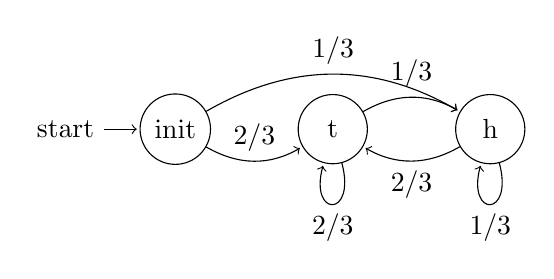
\begin{tikzpicture}[shorten >=1pt, node distance=2cm, on grid, auto]
    \node[state, initial] (q0) {init};
    \node[state] (q1) [right=of q0] {t};
    \node[state] (q2) [right=of q1] {h};
 
    \path[->]
    (q0) edge [bend right] node {2/3} (q1)
    (q0) edge [bend left] node {1/3} (q2)
    (q1) edge [bend left] node {1/3} (q2)
    (q2) edge [loop below] node {1/3} (q2)
    (q2) edge [bend left] node {2/3} (q1)
    (q1) edge [loop below] node {2/3} (q1);
    % (q2) edge [loop above] node {1} (q2);
 \end{tikzpicture}\\
 Now we change this change this chain to fullfil the question.\\
 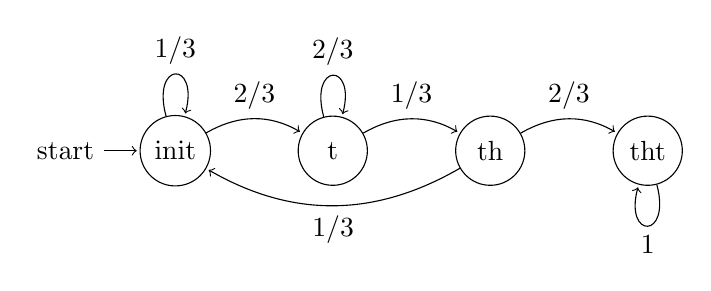
\begin{tikzpicture}[shorten >=1pt, node distance=2cm, on grid, auto]
  \node[state, initial] (q0) {init};
  \node[state] (q1) [right=of q0] {t};
  \node[state] (q2) [right=of q1] {th};
  \node[state] (q3) [right=of q2] {tht};

  \path[->]
  (q0) edge [bend left] node {2/3} (q1)
  (q0) edge [loop above] node {1/3} (q0)
  (q1) edge [bend left] node {1/3} (q2)
  (q1) edge [loop above] node {2/3} (q1)
  (q2) edge [bend left] node {1/3} (q0)
  (q2) edge [bend left] node {2/3} (q3)
  (q3) edge [loop below] node {1} (q3);
  % (q2) edge [loop above] node {1} (q2);
\end{tikzpicture}\\
$E(init) = 1 + 1/3 * E(init) + 2/3 * E(t)$\\\\
$E(t) = 1 + 2/3 * E(t) + 1/3 * E(th)$\\\\
$E(th) = 1 + 2/3 * E(tht) + 1/3 * E(init)$\\\\
$E(tht) = E(init) - 33/4, E(th) = E(init) - 9/2, E(t) = E(init) - 3/2$\\\\
We know that if we get into E(tht), there will remain no step to take $\rightarrow E(tht) = 0$ \\ \\
$E(init) = 33/4, E(th) = 15/4,E(t)=27/4$\\\\
So if we are in init, the expected steps to get to tht would be 33/4 !!!
% $E(tht) = 1 + E(tht)$
%  \begin{equation*}
%    \begin{matrix}
%          &-symp&symp&dead\\\\
%     -symp&\frac{1}{3}&\frac{1}{3}&\frac{1}{3}\\
%     symp&0&\frac{1}{2}&\frac{1}{2}\\
%     dead&0&0&1
%   \end{matrix}
%  \end{equation*}
%  $\pi_{-symp} = 1/3*\pi_{-symp}$\\\\
%  $\pi_{symp} = 1/3*\pi_{-symp} + 1/2 *\pi_{symp}$\\\\
%  $\pi_{dead} = 1/3 * \pi_{-symp} + 1/2 *\pi_{symp} + \pi_{dead}$\\\\
%  $\pi_{dead} + \pi{symp}+\pi_{-symp} = 1 \xrightarrow[]{} \pi_{dead} = 1,\pi_{symp} = \pi_{-symp} = 0$\\\\
%  $E(dead) = 1/3 * E(dead | -symp) + 1/3 * E(dead | symp) *E(symp | -symp)$
\end{latin}